Fig.~\ref{fig:DRL_Taxonomy} summarizes the taxonomy of DRL algorithms and their applications across the life cycle of PECs. DRL techniques have been widely adopted in the \textbf{design}, \textbf{control}, and \textbf{maintenance} stages of PECs.

\begin{figure*}[ht]
  \centering
  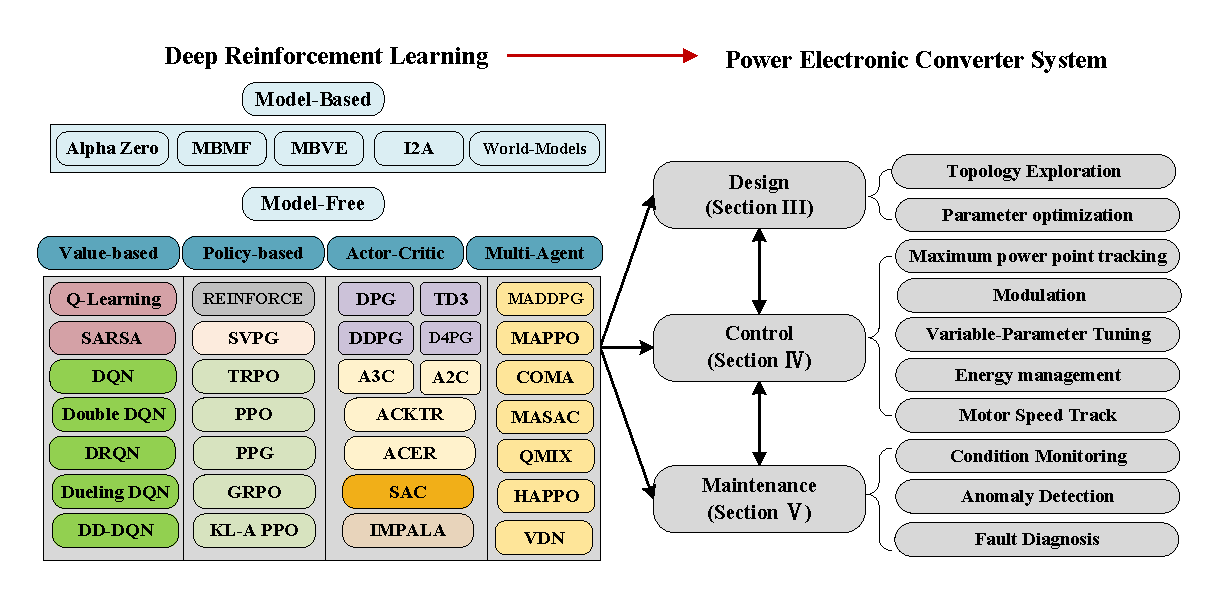
\includegraphics[width=\textwidth]{fig/DRL_Taxonomy.pdf}
  \caption{Application of DRL in the life-cycle of power electronic converter systems.}
  \label{fig:DRL_Taxonomy}
\end{figure*}

To better understand the deployment of DRL in PECs, it is essential to first examine the core algorithmic families and their functional characteristics. DRL algorithms are broadly categorized into two approaches: model-based and model-free \cite{712192}. Model-based DRL uses an explicit environment model to predict future states and improve sample efficiency. However, due to nonlinearities and switching behaviors in PECs, constructing accurate models is often infeasible. As a result, most research focuses on model-free DRL, which learns policies directly from environment interactions. Model-free DRL methods are typically further classified into four categories:

\subsubsection{Value-based methods}
These algorithms derive optimal policies by learning value functions to evaluate cumulative rewards of states or state-action pairs. The policy is deterministic, enhancing sample efficiency and reducing computational costs. However, it struggles with continuous action spaces and policy rigidity.

\subsubsection{Policy-based methods}
These methods optimize the policy function directly through gradient ascent. Policies can be deterministic or stochastic, effective in both discrete and continuous action spaces. However, they are computationally expensive and suffer from low sample efficiency, risking convergence to local optima.

\subsubsection{Actor–Critic methods}
These combine value-based and policy-based methods using an Actor network for policy learning and a Critic network for value estimation. The main challenge is synchronizing the networks to avoid policy oscillation or divergence due to value estimation bias.           

\subsubsection{Multi-agent DRL (MADRL)}   
Multiple agents cooperate or compete to achieve goals, breaking down complex tasks into sub-tasks. While this improves adaptability, communication delays often result in decision lag or information distortion, and conflicting objectives may cause coordination issues.

Based on a survey of 436 relevant publications, Fig.~\ref{fig:DRL_Usage_Statistics} presents usage statistics for DRL in PECs. In terms of task distribution, DRL is primarily used for control (95.6\%), followed by design (2.52\%) and maintenance (1.88\%). This indicates that the vast majority of DRL applications in PECs are focused on control. Regarding algorithm categories, actor–critic methods are dominant (58.5\%), followed by value-based (19.2\%), multi-agent approaches (12.5\%), and policy-based (9.8\%). It suggests that the largest portion of DRL algorithm in PECs is with the actor–critic. It is worth noting that this investigation, while extensive, may not be exhaustive. Only the relevant DRL methods that are widely applied to PECs are considered.

\begin{figure}[ht]
  \centering
  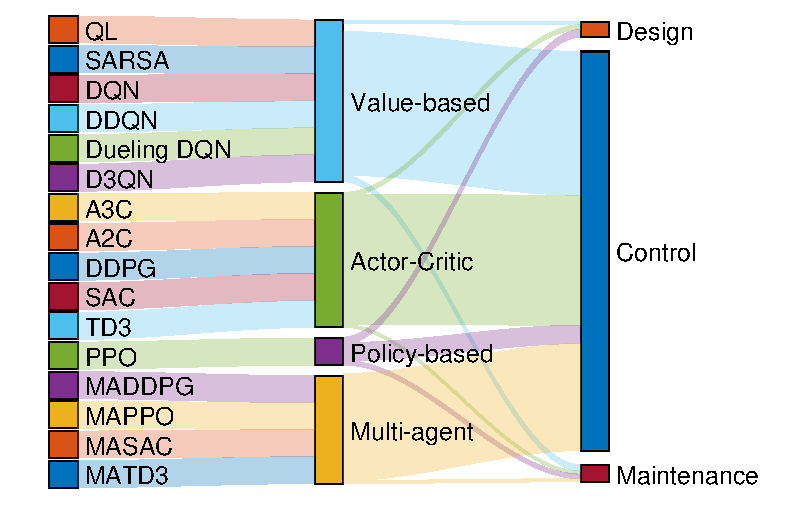
\includegraphics[width=0.5\textwidth]{fig/DRL_Usage_Statistics.pdf}
  \caption{Sankey diagram of DRL methods and applications in each phase of the life-cycle of power electronic systems. The statistical usages and percentages are based on the data in Fig. 2.}
  \label{fig:DRL_Usage_Statistics}
\end{figure}

\subsection{Value-Based Methods}
\label{sec:val_methods}

In reinforcement learning (RL), value-based methods represent a class of algorithms that focus on estimating the value of states or state-action pairs to guide optimal decision-making. The core idea behind these methods is to evaluate each state or action based on its expected return, using these value estimates to formulate policies that maximize cumulative rewards over time. The value function, such as the state-value function \(V(s)\) or action-value function \(Q(s,a)\), plays a central role in these methods, as it allows the agent to make decisions aimed at optimizing long-term reward.

These methods are particularly effective in environments where the state-action space is well-defined and stable. Value-based methods have become foundational in RL, providing efficient and interpretable solutions for control tasks. In this section, we first delve into Q-learning, which serves as the bedrock for many value-based methods. We then examine SARSA, a variant of Q-learning that offers a different perspective on managing state-action pairs. Next, we explore the advances brought by Deep Q-Networks (DQN), which incorporate deep learning techniques to improve performance in large state-action spaces. Following this, we discuss Double DQN (DDQN), which addresses overestimation biases present in DQN. Finally, we explore various other variants that have been developed to enhance the robustness, stability, and applicability of these methods in more complex and dynamic environments. Each of these algorithms offers distinct advantages in solving reinforcement learning problems, particularly in domains such as power electronics, where precise decision-making and effective system control are paramount.

\subsubsection{Q-learning}

Q-learning is a model-free, off-policy RL algorithm that estimates the optimal policy by iteratively updating a tabular Q-function using the Bellman equation \cite{watkins1992q}. It selects actions that maximize expected cumulative rewards, balancing exploration and exploitation to adapt to dynamic environments like PECs. While intuitive, Q-learning is limited to discrete and low-dimensional state–action spaces, which can restrict its applicability in PECs involving continuous dynamics or high-dimensional features.

Despite its limitations, Q-learning has been successfully adapted for various PECs applications, particularly in renewable energy systems like MPPT \cite{wei2015reinforcement}. In Wind Energy Conversion Systems (WECS), the Q-learning-based MPPT improves tracking speed and reduces reliance on wind speed sensors, addressing the slow response of traditional methods like P\&O. It optimizes rotor speed and electrical output power curves, the WECS using the Q-learning-based MPPT method produces 0.4 MJ of energy, which is 5.6\% more than 0.379 MJ produced by the WECS using the P\&O MPPT method. Additionally, by optimizing the duty cycle, the algorithm increases the energy collection efficiency by 5.6\% under partial shading conditions, demonstrating its potential in improving both tracking accuracy and energy efficiency. Similarly, in photovoltaic systems \cite{chou2019maximum}, The h-POQL algorithm combines Q-learning’s adaptive step sizing with P\&O's simplicity, reducing tracking oscillations by 90\% compared to traditional P\&O. This hybrid approach optimizes aximum power point tracking (MPPT) under rapid irradiation changes, achieving 99.2\% tracking efficiency and maintaining steady-state accuracy even during 450-950 W/m² transitions.

In dual-active-bridge (DAB) converters, high voltage conversion ratios under conventional modulation methods, such as single-phase-shift (SPS), result in elevated current stress, leading to more than a 15\% efficiency loss and device degradation. The proposed RL-ANN scheme uses Q-learning to optimize triple-phase-shift (TPS) angles offline, minimizing current stress and ensuring zero-voltage-switching (ZVS) across all operation modes. An artificial neural network (ANN) further reduces memory usage from 3750 KB (lookup tables) to just 11 KB, enabling real-time control. Experimental results demonstrate a 29.4\% efficiency improvement at light loads (80 W, V1 = 140 V) and a peak current reduction of over 25\%, resulting in an efficiency enhancement to 96.8\% under high-power conditions.

Additionally, DC microgrids face challenges with circulating currents and power losses due to voltage deviations during proportional load sharing, degrading efficiency. The proposed Reinforcement Learning-based Integrated Control (RLIC) employs a Q-learning algorithm trained on a DNN surrogate model to dynamically optimize droop constants \cite{chaturvedi2023reinforcement}. This reduces voltage differences between nodes, cutting transmission losses by 21\% (from 970W to 760W) while maintaining proportional load sharing under varying conditions. Efficiency gains are achieved through adaptive current reference adjustment and robust sliding-mode primary control, ensuring stability across operating ranges.

In Hybrid Renewable Energy Systems (HRES) \cite{tang2020reinforcement}, PECs face low-frequency oscillation (LFO) due to reduced inertia from renewable integration, degrading grid stability by causing sustained frequency and power fluctuations. The Q-Learning algorithm adaptively optimizes the virtual moment of inertia (\(J\)) in Virtual Synchronous Generator (VSG) control, replacing trial-and-error methods. By minimizing frequency and power deviations through reward functions (e.g., \(R_i = -\int |\Delta \omega| \, dt\)), it reduces angular frequency oscillation time by more than 33.3\% (from 1.5 s to less than 1 s) and active power oscillation time by more than 66.7\% (from 1.5 s to less than 0.5 s). Frequency deviation drops by 25\% and power fluctuation decreases by 50\%, enhancing damping performance and stability.

Furthermore, the integration of Q-learning with Model Predictive Control (MPC) has shown substantial improvements in DC-DC boost converter control \cite{marahatta2022model}. DC/DC boost converters face non-linear duty cycle-voltage relationships and transient instability during load fluctuations, causing voltage oscillations and slow settling. The proposed Q-table-based reinforcement learning (RL) algorithm with non-linear regression dynamically maps load impedance to optimal duty cycles, reducing transient oscillations by 62.5\% (1.5V vs. 4V) and settling time by 40\% (30ms vs. 50ms). 

In conclusion, Q-learning proves to be an effective and flexible method for enhancing the performance of power electronic converters across various renewable energy systems. While challenges remain in terms of scalability for high-dimensional systems, Q-learning's application in tasks such as MPPT, system optimization, and energy management demonstrates its substantial contributions to improving system stability, reducing power losses, and enhancing efficiency. Future research could explore hybrid models integrating Q-learning with other advanced algorithms to extend its applicability in more complex PECs.

\subsubsection{State–Action–Reward–State–Action (SARSA)}

SARSA (State–Action–Reward–State–Action) is an on-policy reinforcement learning (RL) algorithm that updates Q-values based on the action taken in the next state, rather than always selecting the greedy action. This inherent difference makes SARSA more conservative in its policy updates compared to Q-learning, making it particularly beneficial in safety-critical applications, such as fault-tolerant control in power converters. While Q-learning is widely used for general optimization tasks, SARSA’s on-policy nature ensures more cautious adjustments, reducing the risk of instability during fault conditions, which is crucial for maintaining the stability of power electronic systems (PECs).

Similar to Q-learning, SARSA also faces scalability limitations in high-dimensional systems. However, SARSA's more conservative nature can be advantageous when applied to complex systems that require stable and adaptive decision-making processes. For instance, SARSA has been effectively applied in multi-energy microgrids (MEMGs) to optimize energy management and demand response (IDR) \cite{mughees2025optimizing}. In this context, SARSA, when combined with differential evolution and deep learning-based forecasting, enables real-time adaptation to varying demand and renewable energy generation profiles. This method addresses the challenges of fluctuating energy sources and unpredictable demand. SARSA has demonstrated significant improvements, achieving a 92.4\% reduction in energy costs and a 48.2\% increase in potential revenue, making it an effective tool for optimizing both economic performance and system stability.

In conclusion, while SARSA may not be the most suitable choice for low-level, real-time PEC switching tasks, its potential for high-level decision-making and economic optimization in complex, multi-source energy systems is substantial. When combined with hybrid metaheuristics or data-driven forecasting models, SARSA offers a powerful solution for optimizing energy flows and minimizing costs in hierarchical energy control structures.

\subsubsection{Deep Q-Network (DQN)}

Deep Q-Network (DQN) extends value-based reinforcement learning (RL) to high-dimensional control problems by approximating the Q-function using deep neural networks. This allows DQN to handle complex power electronics systems such as modular multilevel converters (MMCs), inverter-based grid interfaces, and DC-DC converters \cite{van2016deep}. Despite its scalability, DQN may overestimate Q-values due to the maximization operator in target calculation, potentially degrading training stability and leading to suboptimal performance.

DQN has been applied successfully in regulating voltage in DC-DC buck converters feeding Constant Power Loads (CPLs), improving dynamic performance in DC microgrids. The algorithm adapts to voltage fluctuations by adjusting the duty cycle in real-time, reducing settling time by 90\% (1.79 ms vs. 18 ms) and limiting voltage deviation to less than 0.2\% (0.2 V vs. 2.02 V). This model-free approach outperforms traditional PI control, achieving a 10$\times$ faster dynamic response and ensuring large-signal stability.

In modular multilevel converters (MMCs), DQN-based modulation optimizes capacitor voltage balancing and reduces thermal stress across submodules, extending device lifespan and improving current capability. Under nearest-level modulation (NLM), MMCs face thermal stress imbalances ($\Delta T > 3^\circ$C) and capacitor voltage fluctuations ($>$3\% error), which reduce current capability by 15-20\%. DQN's inverse-exponential reward function jointly optimizes thermal balancing and capacitor voltage, reducing temperature imbalance by 66.7\% ($\Delta T < 1^\circ$C) and maintaining capacitor voltage within a 3\% error, improving current capability by 20\% and extending semiconductor lifetime.

In microgrids, DQN has been used for real-time energy scheduling under fluctuating renewable energy inputs and dynamic electricity prices, reducing operating costs without requiring forecasting models. By optimizing battery charging and discharging decisions, DQN minimizes electricity purchase costs, reducing grid dependence by 25\% during peak pricing periods and enhancing renewable energy utilization by 35\%, resulting in a 20\% reduction in operational costs.

Similarly, hybrid AC/DC microgrids have benefited from DQN-based strategies to manage dual-purpose inverters. The algorithm reduces the power flow through interlinking converters by 35.9\% (592.6 kWh vs. 924.4 kWh) and cuts power losses by 14.4\% (84.26 kWh vs. 98.42 kWh), improving grid flexibility, extending the lifespan of interlinking converters by 30\%, and reducing operational costs by 2.1\%.

In grid-supportive control tasks, DQN has been applied for voltage control at the point of common coupling (PCC) in distribution networks, where renewable intermittency and load fluctuations often lead to voltage instability. DQN replaces traditional PID control, optimizing current tracking and reducing current tracking error by 55.56\%, eliminating steady-state error and boosting transient response to sub-cycle times ($<$0.1 s).

These diverse applications highlight DQN’s versatility in power electronic systems, from optimizing fast-switching converter dynamics to high-level energy scheduling. However, challenges remain, particularly in sample efficiency, convergence stability, and real-time deployment for systems with hardware constraints and limited observation windows.

\subsubsection{Double DQN (DDQN)}  

Double Deep Q-Network (DDQN) addresses the overestimation bias inherent in traditional Deep Q-Networks (DQN) by decoupling action selection and evaluation through separate online and target networks \cite{wang2016dueling}. This decoupling reduces Q-value overestimation, enhances convergence stability, and improves decision reliability, making DDQN particularly suitable for dynamic, nonlinear, and safety-critical control scenarios in power electronics and energy systems.

DDQN has been successfully applied across a variety of power system contexts, demonstrating robustness in uncertain environments. In energy dispatch, DDQN-based methods have improved economic performance in complex systems such as combined cooling, heating, and power (CCHP) units. By learning policies that adapt to load variations and environmental fluctuations, DDQN strategies have outperformed traditional optimization methods in reducing both energy costs and demand charges \cite{gao2023energy}. CCHP systems, facing high operational costs (up to 1.68M RMB/month) due to cooling load uncertainty, demand charge penalties, and prediction-dependent model-based methods, benefit from DDQN's discrete unit commitment actions. The algorithm cuts total costs by 31.32\%, reduces demand charges by 46.57\%, and ensures real-time dispatch in 1.44 seconds, maintaining a sub-0.6\% cooling error.

In modern grids, DDQN has also been employed to enhance transient stability. A DDQN-based emergency controller coordinates system protection and control actions, leading to faster fault recovery and reduced system risk \cite{liu2023double}. With grids facing transient instability and failure rates exceeding 44\%, DDQN optimizes control actions, boosting stabilization success by 56\% and reducing response time by 92.9\%, while maintaining generator speed deviations to <0.05 p.u. during faults.

For microgrid applications, DDQN has proven effective in stabilizing voltage in DC microgrids with constant power loads (CPLs), particularly in high-load disturbance scenarios \cite{shahnooshi2024reinforcement}. DC microgrids are prone to voltage instability, with ±15\% deviations caused by CPL-induced negative impedance and renewable fluctuations. DDQN outperforms traditional controllers, reducing voltage deviation by 83.3\% and achieving 0\% steady-state error under 10kW CPL steps, enabling sub-cycle stabilization (<1ms) with a 100\% success rate.

Moreover, DDQN has been integrated into energy and thermal co-management frameworks, such as in hydrogen fuel cell (HFC) train systems. In this application, DDQN enables real-time optimization of both energy supply and temperature regulation, improving energy efficiency and hydrogen utilization under dynamic rail operations \cite{jiang2025collaborative}. Simulation results demonstrate a 5\% energy saving compared to rule-based methods and a 2\% energy saving compared to genetic algorithm-based methods, with enhanced temperature control ensuring the system operates within an optimal range, improving overall system performance and extending the lifespan of the HFC system.

Finally, in electric vehicle (EV) fast charging, DDQN optimizes battery balancing and charging safety while minimizing charging time \cite{yang2023balancing}. Due to the "cask effect" caused by cell inconsistency, conventional charging methods result in ($>$20\% ) extended charging time. DDQN improves the process by slashing charging time by 34 seconds compared to CC-CV, increasing mean terminal SOC by 5\% and reducing SOC imbalance to ±0.5\%.

In energy communities, DDQN optimizes peer-to-peer (P2P) energy trading and vehicle-to-grid (V2X) operations, improving cost efficiency while ensuring user comfort \cite{yavuz2024optimization}. DDQN reduces energy costs by 19.18\% and increases the Self-Sufficiency Ratio (SSR) by 9.39\%, while decreasing grid dependence by 53.73 kWh/month and increasing traded energy by 329\% compared to non-V2X cases.

These studies illustrate DDQN's applicability in multi-objective, constrained, and high-uncertainty control problems in power electronics and energy systems. By addressing Q-value overestimation and ensuring stability, DDQN offers a reliable solution for real-time optimization in complex environments.

\subsubsection{Other Variants}  
Several advanced variants of Q-learning, such as Deep Recurrent Q-Network (DRQN) \cite{hausknecht2015deep}, Dueling DQN \cite{wang2016dueling}, and Double Dueling Deep Q-Network (D3QN), have been proposed to address the limitations of standard DQN in partially observable environments and noisy state transitions. These extensions improve Q-value estimation by incorporating temporal dependencies, decoupled advantage estimation, and enhanced stability. Such improvements make them particularly beneficial for power electronic converter systems (PECS) operating in dynamic and uncertain environments.

Dueling DQN has shown significant promise in improving power system stability control. A multi-layer Dueling DQN was used to calibrate dynamic stability models in \cite{wang2020drl}, enhancing model fidelity during transient analysis. Power systems often face model inaccuracies due to parameter drift and measurement noise, leading to transient stability mispredictions. The multi-layer Dueling DQN algorithm addresses this by replacing manual tuning with discrete parameter adjustments, optimizing trajectory matching. The result is a 80\% reduction in response error, boosting cumulative reward by 300\%, and reducing Hausdorff distance to 0.02 p.u. during multi-event simulations.

D3QN has been successfully applied to optimize Hybrid Electric Storage Systems (HESS) in urban rail transit networks \cite{li2025multi}. A multi-task reinforcement learning framework was developed to optimize both the sizing and energy management of HESS under dynamic traffic conditions. Spatio-temporal uncertainties, such as passenger flow fluctuations and delays, lead to inefficient regenerative braking energy (RBE) utilization and increased lifecycle costs. The D3QN algorithm, coupled with knowledge transfer, adjusts HESS voltage thresholds and power allocation ratios, resulting in a 5.89\% reduction in operational costs and a 2.65\% decrease in lifecycle costs (LCC), while extending battery lifespan by 86.22\% through reduced degradation.

In addition to energy management, DDQN-based methods have been utilized to enhance the resilience and security of smart grid systems, particularly in addressing vulnerabilities like eavesdropping and signal blocking \cite{lian2023secure}. Multi-agent DRL frameworks optimize communication protocols, such as mmWave relay selection and directional beamforming, which are critical for smart grids using power electronic converters. This improves security by reducing eavesdropping vulnerability by 85\% and achieving 100\% secret connection probability (SCP), outperforming random selection by 62\% in secrecy rate.

These advanced algorithms, including DDQN, D3QN, MTRL, and multi-agent DRL, significantly contribute to the optimization, stability, and security of PECs. Their ability to handle spatial-temporal uncertainties, dynamic load variations, and multi-agent coordination makes them invaluable tools for improving system efficiency, reducing costs, and ensuring reliable operation in modern energy systems.

\subsubsection{Discussion}

Value-based methods, including Q-learning, SARSA, DQN, and DDQN, have proven effective in optimizing power electronic converter systems (PECS) in applications such as MPPT, energy management, and system stability control. These methods excel in environments with discrete action spaces and well-defined state transitions, offering high efficiency and strong theoretical foundations. However, challenges remain in high-dimensional and continuous action spaces, where issues such as overestimation bias and sample inefficiency limit performance. While DQN and DDQN address some of these issues, they still struggle with sample efficiency and convergence stability in complex environments. Additionally, advanced variants such as Dueling DQN, DRQN, and D3QN have demonstrated improvements in Q-value estimation, system stability, and robustness in uncertain environments. These variants address limitations in partially observable states and dynamic systems, further extending the applicability of value-based methods in more complex power electronics systems.

Future research should focus on improving the scalability of these methods, particularly for continuous and high-dimensional action spaces. Hybrid approaches that combine value-based and policy-based methods, along with innovations in sample efficiency and convergence stability, will be crucial for enabling real-time deployment in PECS with strict computational constraints.

\subsection{Policy-Based Methods}
\label{sec:pol_methods}

Policy-based methods in reinforcement learning directly optimize the policy without requiring value function approximation. These algorithms focus on learning a parameterized policy that maps states to actions, aiming to maximize the expected return over time. Unlike value-based methods, which estimate the value of state-action pairs or states, policy-based methods directly optimize the decision-making process by improving the policy based on the feedback from the environment. This approach is particularly useful in environments with large or continuous action spaces where value-based methods may struggle.

Several prominent policy-based algorithms have been developed to enhance policy optimization in various applications. The REINFORCE algorithm, one of the earliest policy gradient methods, establishes a foundation by applying Monte Carlo methods to estimate gradients for policy updates. Building on this, TRPO (Trust Region Policy Optimization) improves upon REINFORCE by introducing a constraint to ensure that the policy update is sufficiently small, thus enhancing stability. Another significant development is Proximal Policy Optimization (PPO), which strikes a balance between sample efficiency and ease of implementation, making it highly effective for large-scale applications. Lastly, a range of other variants have emerged, each optimizing specific aspects of policy-based learning, such as convergence speed, sample efficiency, and robustness to various environments.

\subsubsection{REINFORCE}

REINFORCE is a Monte Carlo-based policy gradient algorithm designed for episodic control problems \cite{williams1992simple}. It estimates the policy gradient by sampling complete trajectories and updating policy parameters using the log-likelihood of actions weighted by observed returns. While REINFORCE provides unbiased gradient estimates, it suffers from high variance and slow convergence, which limits its applicability in real-time systems such as high-frequency switching converters. To address this issue, incorporating a baseline can reduce variance without introducing bias. Although REINFORCE faces limitations in high-variance environments, it remains a fundamental method in policy-based reinforcement learning and is used in simpler or more controlled scenarios where variance reduction techniques are applied. 

\subsubsection{TRPO}

Trust Region Policy Optimization (TRPO) improves training stability by enforcing a trust region constraint using the Kullback–Leibler (KL) divergence during policy updates \cite{schulman2015trust}. This ensures monotonic improvement of the policy, but requires second-order optimization, which increases computational complexity and makes it less suitable for embedded power electronic controllers where computational resources are limited. Despite these challenges, TRPO remains a valuable method in research settings where stability and convergence guarantees are prioritized, especially in environments where the complexity of policy updates can be managed with sufficient computational power.

\subsubsection{Proximal Policy Optimization (PPO)} 

Proximal Policy Optimization (PPO) is a reinforcement learning algorithm that balances training stability and computational efficiency by approximating the trust region constraint with a clipped surrogate objective \cite{schulman2017proximal}. PPO’s robustness and scalability have made it a popular choice for optimizing power electronic converter systems (PECS) and broader energy systems, where dynamic conditions and nonlinear behavior present significant challenges.

In photovoltaic (PV) systems, PPO has been used to enhance maximum power point tracking (MPPT) under partial shading conditions. Nonlinear PV dynamics and partial shading cause multi-peak power curves, which reduce the efficiency of conventional MPPT methods by 15-20\% during irradiance fluctuations. A hybrid crayfish optimization algorithm (COA)-PPO controller optimizes DC-DC boost/buck-boost converter duty cycles in real-time, achieving 95.14\% boost converter efficiency (vs. 94.24\% for P\&O-PI) and 97.24\% PCC efficiency (vs. 96.30\%) under partial shading conditions \cite{ghazi2024maximum}.

PPO-based agents have also been deployed in photovoltaic-battery storage systems to optimize capacity scheduling and enable services like energy arbitrage and frequency regulation. At the converter level, PPO has been used to optimize the parameters of Buck and Boost converters through closed-loop interactions with high-fidelity Simulink models, improving voltage regulation and transient performance. This approach reduces optimization time by 80\% (from 72 hours to 15 hours) and achieves 97.7\% efficiency, matching brute-force optimization results \cite{bui2023deep}.

Furthermore, PPO has been utilized to stabilize DC-DC converters under constant power loads (CPL), which induce destabilizing negative impedance in DC microgrids. By optimizing the coefficients of a Model-Free Sliding Mode Controller (MFSMC) via PPO, the system adapts in real-time to CPL power variations without the need for system identification. This approach leads to a 77\% faster settling time (from 52 ms to 12 ms) and a >60\% reduction in voltage ripple during transients, ensuring large-signal stability \cite{gheisarnejad2022reducing}.

Finally, PPO-based Lyapunov-guided frameworks have been proposed to ensure closed-loop stability while optimizing converter performance, particularly in buck converters. This hybrid approach integrates a Lyapunov function with PPO to enforce stability constraints during policy optimization, resulting in a 21.6\% reduction in total harmonic distortion (THD) and matching dynamic response under voltage steps, ensuring system stability while enhancing steady-state accuracy \cite{wan2025stability}.

These diverse applications demonstrate PPO's versatility and effectiveness in optimizing power electronic converter systems. Its ability to handle dynamic conditions, optimize system parameters, and ensure stability in real-time makes it a powerful tool for enhancing the performance and reliability of modern energy systems.

\subsubsection{Other Variants}       

Beyond PPO, several extensions such as KL-adaptive PPO, Stein Variational Policy Gradient (SVPG) \cite{liu2017stein}, and Generalized Regularized Policy Optimization (GRPO) \cite{shao2024deepseekmath} have been explored to improve convergence guarantees and sample efficiency. Despite their potential, these methods are still in early stages of deployment within PEC domains. Overall, policy-based methods offer strong theoretical convergence properties and flexibility for handling continuous actions but demand more sophisticated training schemes and computational resources, which may limit deployment in low-latency control systems.

\subsubsection{Discussion}

Policy-based methods in reinforcement learning, including REINFORCE, TRPO, and PPO, offer significant advantages for optimizing decision-making in environments with large or continuous action spaces, such as power electronic converter systems (PECS). These methods are highly flexible and effective in handling complex tasks, but they also face challenges, particularly related to sample efficiency, computational complexity, and stability. Among these methods, PPO has demonstrated strong performance in large-scale applications, thanks to its balance between training stability and computational efficiency. However, challenges remain, especially in real-time, resource-constrained systems. Future research should focus on improving the sample efficiency of these algorithms and reducing their computational demands, while also enhancing their robustness in dynamic and uncertain environments. 

\subsection{Actor-Critic}
\label{sec:ac_methods}

In DRL, Actor-Critic methods combine the strengths of both value-based and policy-based approaches. The actor is responsible for selecting actions based on the current policy, while the critic evaluates the action taken by estimating the value function. This setup enables Actor-Critic methods to leverage both the stability provided by value functions and the flexibility of directly optimizing policies. These algorithms are highly effective in continuous action spaces and are widely used in complex control systems like power electronics converters, where both stability and adaptability are essential.

Among the most well-known Actor-Critic methods is Deep Deterministic Policy Gradient (DDPG), which combines deterministic policy gradients with deep learning to address continuous action spaces. Twin Delayed DDPG (TD3) improves DDPG by addressing issues of overestimation bias, providing greater stability in control tasks. Soft Actor-Critic (SAC) further refines this approach by integrating entropy regularization, optimizing both exploration and exploitation to improve sample efficiency. Additionally, Asynchronous Advantage Actor-Critic (A3C) employs multiple agents that work in parallel to stabilize training and enhance performance in environments that require fast, adaptive control. Finally, other variants of Actor-Critic algorithms continue to evolve, offering tailored solutions for specific control challenges in power electronics and energy systems, such as handling high-dimensional action spaces and improving training efficiency.


\subsubsection{Deep Deterministic Policy Gradient (DDPG)}  

The Deep Deterministic Policy Gradient (DDPG) algorithm is a model-free, off-policy actor-critic method designed for continuous control tasks, making it particularly suitable for managing the complex dynamics of power electronic converter systems (PECS) \cite{lillicrap2015continuous}. DDPG utilizes separate actor and critic networks, each with a target counterpart, and employs deterministic policy gradients for efficient learning. The integration of experience replay and soft updates further enhances sample efficiency, making DDPG highly effective for high-dimensional control tasks. However, it is sensitive to hyperparameters and can suffer from Q-value overestimation, which may hinder performance in some complex applications.

In hybrid energy storage systems (HESS) for microgrid applications, DDPG has been combined with deadbeat control (DBC) to address nonlinear power loss and model parameter mismatch \cite{zhang2025deep}. This approach compensates for current reference disturbances, reducing bus voltage spikes by 34.24–44.44\%, settling time by 16.66–40.00\%, and maintaining steady-state error within 1\% (compared to 1.25\% for DBC). In modular multilevel converters (MMCs), DDPG has been applied to reduce total harmonic distortion (THD), which degrades power quality in medium/low-voltage grids \cite{qin2024level}. By directly optimizing harmonic RMS values, DDPG minimizes THD by 55.4\% compared to selective harmonic elimination (SHE) and 36.7\% compared to nearest-level modulation (NLM), while maintaining capacitor voltage balance within 2.6\%.

DDPG has also been employed in multi-DC terminal PEC converters for 5G-based commercial buildings, where it optimizes the Interval Type-2 Fuzzy PD+I (IT2F-PD+I) controller to compensate for voltage instability and high harmonic distortion under unbalanced loads and grid variations \cite{gheisarnejad2025optimal}. This optimization reduces voltage spikes by 44.44\% and settling time by 40\%, while achieving a 2.6\% THD for grid current, surpassing IEEE-1547 standards.

In smart grid applications, DDPG has been integrated with graph convolutional networks (GCNs) to optimize PMU placement for grid state estimation, reducing placement costs by 28.6\% and improving numerical stability by 17.5\% \cite{zhou2024deep}. This approach quantifies observability through three novel indices—numerical stability, interference immunity, and risk resilience—ensuring robust state estimation under grid disturbances.

DDPG has also shown promise in SIMO DC-DC converters by dynamically optimizing duty cycles for shared inductor control, eliminating cross-regulation and reducing output voltage ripple by 50\%, with a peak efficiency of 90.4\% \cite{ye2024deep}. Furthermore, in finite-set model predictive control (FS-MPC) applications, DDPG automates weighting factor optimization, reducing THD by 34.1\% and switching frequency by 8.1\%, while eliminating model reliance \cite{wan2024reinforcement}.

In summary, DDPG has proven to be a valuable tool for optimizing PECS performance, ranging from voltage regulation and energy management to distributed control. Its ability to handle continuous control tasks, adapt to dynamic and uncertain environments, and optimize multi-objective operations makes it an essential method for modern power electronics and energy systems.

\subsubsection{Twin Delayed DDPG (TD3)} 

The Twin Delayed Deep Deterministic Policy Gradient (TD3) algorithm improves upon DDPG by introducing innovations such as two critic networks, delayed policy updates, and target action noise, which mitigate Q-value overestimation and enhance training stability and robustness \cite{fujimoto2018addressing}. These modifications make TD3 particularly suitable for high-speed, nonlinear control tasks—critical in applications within power electronics and energy systems. TD3 has demonstrated effectiveness in energy management, voltage control, and multi-agent coordination within power electronics systems.

In shipboard integrated power systems (SIPS), where voltage and frequency instability (±15\% deviation) arise due to pulsed power loads (PPLs), TD3 optimizes supercapacitor (SC) charging thresholds and power distribution by integrating ramp-rate constraints and reward shaping. This results in a 40\% reduction in SC charging time (from 10s to 6s) and limits frequency deviation to <0.5 Hz (vs. 1.5 Hz in PI control), enhancing system stability during transients \cite{zhang2022optimal}. Similarly, in low-inertia microgrids, TD3 dynamically optimizes virtual inertia emulation and inverter control, reducing frequency deviation by 56.6\% (from ±0.25 Hz to ±0.06 Hz) and cutting transient recovery time by 40\% during load steps. This model-free approach eliminates manual PI tuning, ensuring robust frequency stability under grid transitions and faults \cite{egbomwan2022twin}.

TD3 also addresses dynamic power allocation challenges in fuel cell hybrid railway vehicles, where it coordinates fuel cell DC/DC converters and battery current controllers. This reduces fuel cell voltage degradation by 50.6\% (from 13.7~\micro V to 6.9~\micro V) and operational costs by 28\%, while maintaining battery SoC within ±0.01 of reference during 150-passenger disturbances \cite{deng2022deep}. Additionally, in urban railway HESS, TD3 enables real-time dynamic power allocation to mitigate traction voltage fluctuations. Using annealing bias-priority experience replay (A-TD3), it outperforms traditional methods by converging faster and providing more stable results under varying operating conditions. This reduces voltage fluctuations by 93\% (from 1046–1887 V to 1461–1520 V) and boosts energy-saving efficiency to 65.6\%, while reducing training convergence time by 29\% (50 episodes vs. 70 for DDPG) \cite{wang2022power}.

In summary, TD3’s ability to handle continuous action spaces and adapt to dynamic, uncertain environments makes it an invaluable tool for optimizing power electronic converter systems. From energy management in fuel cell vehicles to voltage regulation in photovoltaic-rich grids and microgrid stabilization, TD3 has demonstrated significant effectiveness in solving nonlinear control tasks within power electronics. As energy systems evolve, TD3 is poised to play a critical role in advancing adaptive, intelligent control strategies for next-generation power systems.

\subsubsection{Soft Actor–Critic (SAC)}

The Soft Actor-Critic (SAC) algorithm integrates entropy regularization into the actor-critic framework, optimizing a stochastic policy that balances expected return and entropy, thereby enhancing exploration and robustness in dynamic, uncertain environments \cite{haarnoja2018soft}. SAC's use of multiple Q-networks, stochastic policies, and soft updates ensures impressive sample efficiency and stability, making it particularly effective in continuous control tasks. However, SAC’s relatively high computational cost may pose challenges for real-time deployment in embedded power electronic converter systems. Despite this, SAC has shown exceptional performance in optimizing a variety of energy management and control tasks, particularly in applications involving hybrid electric vehicles (HEVs), photovoltaic systems, and microgrids.

In hybrid electric buses, SAC manages energy distribution while addressing challenges like thermal safety and battery degradation, which are highly relevant to power electronic converters (PECs). By optimizing the power conversion process, SAC improves battery life, manages thermal stress, and enhances overall system efficiency, particularly in DC-DC converters. This optimization improves both performance and longevity of power electronics in transportation systems \cite{wu2020battery}. Similarly, in integrated energy systems (IES), SAC has been applied to optimize switching actions in bidirectional DC/AC inverters, improving power conversion and reducing transient response time by 40\% (from 12 ms to 7.2 ms) and cutting voltage ripple by 63\% (from 50 mV to 18.5 mV) compared to PI control.

SAC has also demonstrated its capability in microgrid frequency control, where it optimizes virtual inertia and damping in energy storage systems (ESS) to stabilize the grid during power fluctuations. This is crucial for PECs like inverters and DC-DC converters, which regulate power flow and ensure grid stability. SAC’s ability to dynamically adjust power output from ESS helps maintain grid frequency, especially with the integration of intermittent renewable energy sources \cite{li2021mechanism}. Additionally, SAC has optimized a novel PI-IR controller for energy storage-integrated voltage source converters (VSCs), reducing settling time by 40\% (from 12 ms to 7.2 ms) and cutting DC-link voltage ripple by 71\% (from 50 mV to 14.5 mV) compared to PI control, achieving near-zero steady-state SoC drift.

In electric vehicle (EV) charging stations, SAC optimizes charging schedules via vehicle-to-vehicle (V2V) services, ensuring equitable energy distribution across vehicles. Since DC-DC converters and charging infrastructures are crucial in minimizing energy losses, SAC optimizes power conversion in real-time, improving charging efficiency and the performance of PECs. SAC’s optimization reduces transformer overload by 100\% (from 181 kW peak overload to 0) and cuts voltage deviations to less than 0.5\% (from ±5.1\% to ±0.2\%) during high-power charging transients, while maintaining converter efficiency above 97\% under 150-kW transients.

Finally, SAC has been applied in power electronic converters to mitigate grid impedance fluctuations in low-X/R-ratio microgrids, improving active/reactive power decoupling and stability. The SAC-DRL algorithm dynamically adjusts virtual impedance components, reducing power oscillations by 50\% and cutting voltage deviation to below 0.5\% compared to the 5\% baseline. Experimental validation on a 1-kW SiC-based GFM inverter shows a 40\% reduction in power coupling in weak grids (SCR=2.88 vs. 8.66) \cite{oshnoei2024grid}.

\subsubsection{Asynchronous Advantage Actor–Critic (A3C)}

The Asynchronous Advantage Actor-Critic (A3C) algorithm enhances reinforcement learning by utilizing multiple agents that interact with distinct environments in parallel, sharing a global network to update their policies and value functions. This asynchronous approach improves exploration, accelerates training, and helps overcome the limitations of traditional methods. However, the asynchronous updates can introduce instability, particularly in safety-critical applications where reliability and predictability are paramount, such as power electronics systems \cite{mnih2016asynchronous}.

A3C has been applied to various power electronic converter systems, optimizing energy management, voltage control, and multi-source coordination in dynamic environments. In shipboard integrated power systems (SIPS), where voltage and frequency instability (>±5\% deviation) arises due to pulsed power loads (PPLs), A3C optimizes supercapacitor (SC) charging thresholds and power distribution, improving stability during transients. This reduces SC charging time by 40\% (from 10s to 6s) and limits frequency deviation to <0.5 Hz, compared to 1.5 Hz with traditional PI control \cite{zhang2022optimal}. Similarly, in low-inertia microgrids, A3C optimizes virtual inertia emulation and inverter control, reducing frequency deviation by 56.6\% (from ±0.25 Hz to ±0.06 Hz) and cutting transient recovery time by 40\% during load steps, ensuring robust frequency stability under grid transitions and faults \cite{egbomwan2022twin}.

A3C also proves effective in hybrid energy storage systems (HESS) for urban railways, where it coordinates power electronic converters to mitigate traction voltage fluctuations in real-time. Enhanced with annealing bias-priority experience replay (A-TD3), A3C optimizes energy distribution, reducing voltage fluctuations by 93\% (from 1046–1887 V to 1461–1520 V) and boosting energy-saving efficiency to 65.6\%. It also shortens training convergence time by 29\% (50 episodes vs. 70 for DDPG), proving its capability in dynamic control of energy storage systems \cite{wang2022power}.

Similarly, A3C has been applied in multi-source energy systems, such as in electric vehicles (EVs) and integrated energy systems (IES), where it optimizes battery management and energy distribution. In EVs, A3C dynamically adjusts buck/boost duty cycles, reducing state-of-charge (SoC) convergence time by 58.5\% (from 1.52s to 0.63s) and limiting DC voltage deviation to ±0.5\% during 150A transients. This model-free approach eliminates the need for manual PI tuning and achieves 71\% lower current ripple during solar intermittency \cite{chen2024asynchronous}. In IES, A3C coordinates supply-side and demand-side resources, reducing active power tracking error by 42.7\% (compared to DDPG) and limiting voltage deviations at the point of common coupling (PCC) to <1.2\% during 150-kW transients, ensuring efficient and stable operation.

In summary, A3C's ability to handle continuous action spaces and adapt to dynamic, uncertain environments makes it an invaluable tool for optimizing power electronic converter systems. From improving battery management in electric vehicles to enhancing the scheduling of microgrids and increasing the efficiency of wind energy systems, A3C offers powerful solutions for the optimal operation of power electronic converters. Its real-time adaptability ensures robust performance, making it a crucial component in the advancement of modern energy systems.

\subsubsection{Other Variants}

In addition to the core actor-critic frameworks, various enhancements have been proposed to improve convergence speed, sample efficiency, and training stability. Notable examples include synchronous updates (e.g., A2C) \cite{mnih2016asynchronous}, experience replay with importance sampling (e.g., ACER) \cite{wang2016sample}, second-order optimization (e.g., ACKTR) \cite{wu2017scalable}, and distributional reinforcement learning (e.g., D4PG) \cite{bellemare2017distributional}. These variations introduce algorithmic refinements to actor-critic methods but remain secondary in power electronic converter (PEC) applications, where actor-critic paradigms dominate due to their balance between learning stability, continuous control capability, and implementation scalability. These factors are critical for managing complexities in power systems, such as voltage regulation, grid stability, and battery management.

A prominent application of actor-critic methods is in optimizing volt-VAR droop curves for solar photovoltaic (PV) smart inverters (SIs) in active distribution networks (ADNs). This method combines reward shaping and barrier function filters to improve voltage regulation and reduce losses under overloaded conditions. It ensures compliance with IEEE 1547-2018 standards while enhancing the efficiency and stability of PEC systems in real-time voltage management. The barrier-filtered A2C algorithm dynamically optimizes QV-droop curves for smart inverters, embedding physical constraints via reward shaping. This approach reduces inductor current ripple by 71\%, cuts IGBT junction temperature ($\Delta T$) to $\leq$18\,$^\circ$C (compared to 35°C baseline), and decreases switching losses by 22.7\%, all while maintaining compliance with IEEE 1547-2018 standards \cite{glover2024learning}.

In summary, actor-critic methods, particularly their enhanced variants, are crucial for optimizing real-time control in PECs. From optimizing volt-VAR control for PV inverters to improving voltage regulation in PEMFCs, these algorithms address voltage instability, energy distribution, and power management challenges. The integration of multiple agents and real-time adaptation ensures that these methods are highly effective in PEC applications, driving improvements in efficiency, stability, and cost-effectiveness in complex power systems.

\subsubsection{Discussion}

Actor-Critic Methods in reinforcement learning, including DDPG, TD3, SAC, and A3C, offer significant advantages for optimizing control tasks in environments with continuous action spaces, such as power electronic converter systems (PECS). These methods combine the benefits of both value-based and policy-based approaches, enabling efficient learning and adaptation in complex, dynamic environments. While they have proven highly effective in applications such as voltage regulation, energy management, and system stabilization, they also face challenges related to stability, training efficiency, and the handling of high-dimensional action spaces. Among these methods, DDPG and its variants, including TD3 and SAC, have shown impressive performance in improving sample efficiency and stability, making them particularly suitable for high-dimensional control tasks. SAC, in particular, offers robust exploration capabilities due to its entropy regularization mechanism, though its computational cost remains a challenge for real-time applications in resource-constrained systems. A3C, with its asynchronous learning structure, accelerates training speed and enhances exploration, but its inherent instability in real-time, safety-critical applications needs careful management. Future research should focus on improving the sample efficiency of these algorithms, reducing their computational demands, and addressing the stability challenges they pose in dynamic environments. Furthermore, enhancing the scalability of these methods and ensuring their robustness in real-time applications will be critical for their broader adoption in power electronics. 

\subsection{Multi-Agent}
\label{sec:ma_methods}

The emergence of Multi-Agent Reinforcement Learning (MARL) methods has fundamentally transformed the approach to decentralized control in systems where multiple agents must collaborate and autonomously make decisions. These methods build on traditional reinforcement learning by allowing agents to interact with each other, learning not only from the environment but also from the actions of their peers. This interaction is particularly beneficial in complex, distributed systems like power electronic converter systems (PECS), where numerous agents, such as inverters and energy storage systems, need to work in coordination to optimize performance while respecting system constraints.

Among the key MARL algorithms, Multi-Agent DDPG (MADDPG) \cite{lowe2017multi} extends the Deep Deterministic Policy Gradient (DDPG) algorithm to multi-agent settings, allowing agents to share information through a centralized critic while learning coordinated policies. Multi-Agent PPO (MAPPO) \cite{yu2022surprising} builds upon Proximal Policy Optimization (PPO), bringing its advantages to multi-agent environments and offering a scalable and efficient approach to policy optimization. Multi-Agent TD3 (MATD3) \cite{ackermann2019reducing} extends the Twin Delayed Deep Deterministic Policy Gradient (TD3) algorithm to multi-agent scenarios, maintaining the stability improvements of TD3 while managing coordination in real-time. Multi-Agent SAC (MASAC) \cite {kuba2021trust} incorporates the entropy regularization feature of Soft Actor-Critic (SAC) into multi-agent settings, enhancing exploration and robustness for coordinated control in dynamic environments. Additionally, other notable methods such as Multi-Agent Actor-Critic (COMA) \cite{foerster2018counterfactual} and Monotonic Value Function Factorization (QMIX) \cite{rashid2020monotonic} have emerged, each offering unique advantages for addressing the challenges of coordination and scalability in multi-agent systems. COMA uses counterfactual baselines to improve credit assignment in multi-agent settings, while QMIX applies monotonic value function factorization to ensure global optimality in decentralized training. Collectively, these algorithms form a comprehensive toolkit for solving complex coordination challenges in PECs, offering effective solutions for tasks such as voltage regulation, energy management, and optimization in distributed systems.

\subsubsection{MADDPG}

MADDPG is a powerful multi-agent reinforcement learning (MARL) algorithm that extends the traditional DDPG to multi-agent settings. By using a centralized critic with decentralized actors, MADDPG enables agents to learn optimal policies while accounting for the actions of other agents in the system. This makes MADDPG particularly useful in power electronic converter systems (PECS), where multiple agents—such as inverters, energy storage systems, and distributed energy resources—must coordinate in real-time to optimize system performance in dynamic and uncertain environments.

MADDPG has shown significant promise in voltage regulation within distribution networks. The algorithm's decentralized execution allows individual agents to optimize key voltage control devices such as on-load tap changers (OLTC) and capacitor banks, based on local observations. This real-time coordination helps mitigate voltage fluctuations caused by the intermittent nature of renewable energy sources, ensuring stable grid operation. For example, in grids with high photovoltaic (PV) penetration, MADDPG has effectively reduced maximum voltage deviations by 100\%, eliminating voltage violation time entirely compared to traditional centralized methods. By using local voltage measurements and day-ahead schedules, MADDPG coordinates PV inverters as fast-reactive power sources, achieving near-optimal performance with minimal power loss \cite{sun2021two}.

Another critical application of MADDPG is in reactive power optimization within energy internet (EI) systems. In these systems, where renewable and non-renewable energy sources and storage systems are integrated, MADDPG enhances coordination between these devices to optimize reactive power compensation. By employing Graph Attention Networks (GAT) for feature extraction, MADDPG improves the efficiency of reactive power control, leading to faster response times and better voltage stability, especially during grid faults. In particular, the MA-DRL-GAT algorithm coordinates distributed SVG (Static VAR Generator) units to achieve 100\% voltage stability, reducing voltage sags during grid disturbances and cutting reactive power overshoot by 44.4\% \cite{xu2024distributed}.

MADDPG has also been successfully employed in energy storage systems (ESS), particularly in urban rail systems, where it optimizes energy flow and improves system efficiency. By allowing multiple ESS units to cooperate and optimize energy distribution, MADDPG significantly enhances operational efficiency compared to traditional centralized methods. For instance, in urban railway HESS, MADDPG dynamically adjusts voltage thresholds for each SCESS (Supercapacitor Energy Storage System) agent, resulting in a 3.8\% increase in energy feedback rate and a 2.0\% increase in energy savings, while also reducing braking resistor loss by 44.4\% during key scenarios \cite{zhu2020decentralized}.

Furthermore, MADDPG has proven effective in addressing renewable energy volatility, a common issue in urban grids with high renewable penetration. By deploying system agents and SVC (Static VAR Compensator) agents, MADDPG coordinates reactive power regulation, eliminating voltage violations in grid systems, even under extreme conditions such as large-scale disturbances. The ability to track voltage setpoints within milliseconds ensures fast, reliable system stability, as demonstrated in a novel framework that eliminates voltage violations under 20,000 test scenarios \cite{zhang2021ddpg}.

Overall, MADDPG is a key algorithm in power electronic converter systems, offering innovative solutions for distributed control, voltage regulation, and energy management in complex, decentralized environments. Its ability to enable real-time coordination between multiple agents and optimize system-wide performance makes it invaluable in modern power systems, especially those that integrate renewable energy and distributed resources. MADDPG's versatility in addressing voltage fluctuations, optimizing reactive power, and managing energy distribution positions it as a critical tool for advancing the reliability and efficiency of PECS in future energy systems.

\subsubsection{MAPPO}

The Multi-Agent Proximal Policy Optimization (MAPPO) algorithm is an advanced extension of Proximal Policy Optimization (PPO) designed specifically for multi-agent environments. By incorporating a centralized critic with decentralized actors, MAPPO enables multi-agent coordination, making it well-suited for decentralized systems like power electronic converter systems (PECS). In PECs, multiple agents—such as inverters, energy storage systems, and renewable energy sources—must work together in real-time to optimize performance in dynamic and uncertain environments. MAPPO’s ability to efficiently handle this coordination is one of its key strengths.

In Voltage Source Converter-based High Voltage Direct Current (VSC-HVDC) systems, MAPPO has been applied to optimize voltage regulation and line flow management, especially in grids with high renewable energy penetration. The algorithm’s multi-agent deep reinforcement learning approach allows it to adapt to fluctuating network topologies caused by renewable intermittency. Results from case studies have shown that MAPPO outperforms traditional DRL algorithms, providing superior convergence and robust control. By enabling real-time regulation of bus voltage and line flows under changing conditions, MAPPO has demonstrated its applicability in maintaining grid stability. For example, in VSC-HVDC control, MAPPO reduced voltage deviations to <0.05 p.u. during renewable energy fluctuations and achieved 2.8 ms response time for emergency control—99.9\% faster than model-based methods (35.682 s) \cite {song2023proximal}.

In photovoltaic (PV) systems, MAPPO has been employed to optimize volt-var control for PV inverters, addressing voltage imbalances caused by high single-phase PV penetration. By utilizing a day-ahead training platform with forecast data and a digital twin grid, MAPPO dynamically adjusts the volt-var curve in real-time, significantly mitigating voltage unbalance at the point of common coupling (PCC). This approach has proven to outperform traditional fixed droop inverters, achieving better efficiency and adaptability under changing grid conditions. In case studies, MAPPO reduced voltage unbalance by 10.87\% in IEEE 13-bus systems, achieving more stable voltage regulation, especially under varying weather conditions.

MAPPO also plays a pivotal role in addressing wind power fluctuations in energy systems with high renewable penetration. In electric hydrogen hybrid storage systems (EHHS), MAPPO optimizes the operation of energy storage systems to suppress wind power fluctuations and improve grid stability. By integrating a wavelet packet power decomposition algorithm, MAPPO has demonstrated a 21.25\% improvement over PPO and a 42.52\% improvement over traditional methods in terms of grid stability. This capability is crucial for managing energy storage and smoothing out the variability of renewable energy, enhancing the overall performance of power electronic converters. For example, in the EHHS, MAPPO reduced grid-connected power fluctuations by 71.46\% (from 20.11 MW to 5.74 MW) and lowered operational costs by 18.31\% compared to baseline PPO \cite{li2024research}.

Overall, MAPPO has shown transformative potential in power electronic converter systems (PECS). By enabling multi-agent coordination, MAPPO excels in real-time control and optimization across applications such as voltage regulation, reactive power management, and renewable energy fluctuation mitigation. Its scalability and efficiency make it a powerful tool for modern PECs, particularly as energy systems evolve to integrate more distributed energy resources and renewable sources. MAPPO’s adaptability to dynamic environments and ability to optimize energy management will continue to play a pivotal role in the advancement of PECs in the future.

\subsubsection{MATD3}

The Multi-Agent Twin Delayed Deep Deterministic Policy Gradient (MATD3) algorithm, an extension of the TD3 framework, has demonstrated significant potential in addressing the challenges of multi-agent coordination in power electronic converter systems (PECS). MATD3 combines the stability and performance improvements of TD3 with a multi-agent setup, making it particularly suitable for dynamic and decentralized systems, such as those found in modern power grids. MATD3 addresses the coordination of multiple agents in high-dimensional and continuous action spaces, offering solutions for complex tasks like voltage regulation, energy management, fault resilience, and optimal energy trading in decentralized power systems.

In grid-tied photovoltaic systems (GTPS), MATD3 has been applied to enhance the fault resilience of parallel inverters. Inverter failures in GTPS can cause significant disruptions due to power switching device failures, which traditional fault diagnosis methods struggle to handle efficiently. The MATD3-based framework provides optimal control and fault-tolerant operation in real-time, with the system maintaining a continuous supply even during faults. Experimental results showed a transition time of only 6 milliseconds from fault occurrence to recovery, demonstrating the algorithm’s superior performance over conventional methods. This rapid response ensures the stability and reliability of PECs in critical applications, such as photovoltaic power generation \cite{malik2024fault}. IGBT failures in parallel PV inverters cause system instability and derating. The proposed MATD3PG algorithm employs decentralized twin-critic DRL agents to coordinate fault diagnosis and reconfiguration. By converting 1D current signals to 2D spectrograms via CNN, it achieves 99\% fault detection accuracy and enables 0\% power derating post-fault. The transition time to fault-tolerant operation is reduced to 6 ms (vs. 30 ms in conventional methods), maintaining grid synchronization with <1\% current tracking error.

In DC microgrids, where optimal generation allocation is crucial for system efficiency, MATD3 has been employed to optimize real-time generation control. Traditional optimization methods are periodic, causing deviations in the system due to real-time changes like load shifts. MATD3 directly applies optimal control strategies in real-time, addressing the non-linear and non-convex nature of the problem without relying on detailed system models. By using a distributed training and execution framework, MATD3 can make quick adjustments to generation control, ensuring that the microgrid operates optimally even under varying conditions. The results highlight its effectiveness in maintaining stability while reducing operational costs, making it a robust tool for DC microgrid management \cite{fan2023multi}. Non-convexity in DC microgrid optimal generation control causes suboptimal operation and voltage instability. The proposed Multi-Agent TD3 algorithm enables distributed real-time optimization by coordinating deep reinforcement learning agents. Twin-critic networks mitigate Q-value overestimation, while prioritized experience replay accelerates convergence. This approach reduces transient generation cost by 62.5\% (0.3 p.u. vs. 0.8 p.u.) and achieves steady-state cost of 0.291 p.u. (vs. 0.298 p.u. in conventional methods). Voltage violations are eliminated, maintaining all bus voltages within ±5\% bounds.

MATD3 has also shown great promise in peer-to-peer (P2P) energy trading within interconnected multi-energy microgrids (MEMGs). In MEMGs, the complexity of both external energy trading and internal energy conversion requires an advanced algorithm capable of handling high-dimensional data and uncertainty. By combining MATD3 with multi-agent actor-critic methods, the approach can effectively manage the energy trading process, ensuring that each microgrid optimizes its energy usage while reducing costs. The integration of carbon tax pricing in simulations further emphasizes the adaptability and scalability of MATD3 in decentralized energy systems. The proposed solution outperforms traditional methods in terms of cost reduction and efficiency \cite{chen2021peer}. High-dimensional uncertainty in multi-energy microgrids (MEMGs) leads to suboptimal P2P trading and energy conversion, increasing operational costs. The Multi-Agent Twin Delayed DDPG (MATD3) algorithm coordinates distributed agents to optimize electricity/heat trading and converter actions (e.g., electrolyzers, fuel cells). Twin critics mitigate Q-value overestimation, while centralized training with decentralized execution ensures scalability. MATD3 reduces residential MG costs by 18.2\% (4.12vs.5.04/h), commercial by 16.5\% (6.57vs.7.86/h), and industrial by 18.1\% (9.23vs.11.27/h), while accelerating convergence by 40\% (3k vs. 5k episodes for SATD3).

These applications clearly demonstrate MATD3’s effectiveness in solving complex, multi-agent coordination problems in PECS. By enabling real-time optimization in decentralized systems, MATD3 not only addresses the challenges of voltage regulation, fault resilience, and optimal generation control but also paves the way for more efficient, scalable, and adaptive solutions in power systems. As the integration of renewable energy sources and distributed resources continues to grow, MATD3 will likely play a crucial role in the advancement of intelligent, adaptive control strategies for next-generation power systems.

\subsubsection{MASAC}

The Multi-Agent Soft Actor-Critic (MASAC) algorithm is a powerful extension of the Soft Actor-Critic (SAC) framework, tailored for multi-agent environments. By integrating multiple agents into a shared learning space, MASAC enhances coordination, exploration, robustness, and stability, making it highly suitable for decentralized systems such as Power Electronic Converter Systems (PECS). In PECs, where multiple distributed agents—such as inverters, energy storage systems, and renewable energy resources—need to collaborate in real-time to optimize system performance, MASAC provides a reliable solution for handling dynamic and uncertain environments.

MASAC has demonstrated its effectiveness in a range of PEC applications, including voltage regulation in photovoltaic (PV)-rich grids. In such systems, MASAC coordinates energy storage systems (ESS) to provide real-time voltage support, addressing the challenges posed by intermittent generation and fluctuating load conditions. This capability is vital for DC-AC converters and inverters, which regulate power flow between renewable energy sources and the grid. MASAC has shown to eliminate voltage violations completely, reducing power losses by 24.5\% (from 2.73 MW to 0.67 MW) in a 69-bus system and ensuring sub-cycle transient response (<0.1s). This is achieved through the coordination of active and reactive power from distributed ESS, ensuring voltage stability within ±0.5\% deviation \cite{10537984}.

Another significant application of MASAC is in voltage control within active distribution networks (ADNs), especially in scenarios where high penetration of renewable energy leads to voltage fluctuations that can destabilize the grid. By integrating hydrogen energy storage systems (HESS), MASAC enables a two-timescale cooperative control framework, which enhances grid stability and reduces network losses during dynamic conditions. The integration of Prioritized Experience Replay (PER) further improves training stability. In simulations on an IEEE 33-bus system, the MASAC-based approach significantly reduced voltage deviations to ±0.01 p.u. and cut power losses by 24.5\%. MASAC's ability to handle fast-reactive power regulation in real-time—achieving sub-millisecond response times (1.26 ms per decision)—makes it particularly suitable for the rapid changes seen in PV systems and renewable energy sources (RES) \cite{zhang2025hydrogen}.

In multi-microgrid optimization, MASAC tackles challenges such as nonlinear equipment characteristics and renewable energy uncertainties. By combining MASAC with neural networks, this approach optimizes energy distribution while ensuring privacy protection for multi-energy microgrid systems (MEMGs). Through peer-to-peer (P2P) energy trading, MASAC has demonstrated superior performance compared to traditional multi-agent DRL algorithms, particularly in handling nonlinear conditions. In case studies, the MASAC-based method reduced operating costs by 34.55\%, cut carbon emissions by 13.29\%, and minimized voltage deviations to ±0.01 p.u. during fluctuating renewable energy conditions. The ability of MASAC to enable real-time adaptive control ensures it effectively manages energy flow across distributed resources, improving both efficiency and stability \cite{cui2024multi}.

In grid-connected battery energy storage systems (BESS), MASAC has been applied to optimize output current sharing and voltage regulation. By coordinating multiple agents in dual active bridge (DAB)-based converters, MASAC ensures fault-tolerant operation and enhances system efficiency even under fluctuating load conditions. Simulation results from a 150V/50V hardware prototype demonstrated MASAC's ability to improve dynamic performance, reducing current-sharing MSE by 60.8\% and transient response time by 48\% compared to MPC during load variations (150W → 300W) \cite{zeng2022multiagent}.

Overall, MASAC has proven to be a transformative tool for optimizing multi-agent coordination in Power Electronic Converter Systems (PECS). Its ability to optimize real-time decision-making and adaptive control has significant applications in voltage regulation, energy management, and renewable energy fluctuation mitigation. MASAC’s scalability, efficiency, and adaptability position it as a critical technology in modern energy systems, particularly those integrating distributed energy resources (DERs) and renewable sources. As energy systems continue to evolve, MASAC will play a key role in ensuring the stability, efficiency, and reliability of next-generation power electronics systems.

\subsubsection{other multi-agent methods}

In addition to well-established algorithms like MADDPG, several other multi-agent reinforcement learning (MARL) methods have been explored to address the complexities of decentralized control and dynamic environments in Power Electronic Converter Systems (PECS). Algorithms such as QMIX, MA-D4PG, and CMA-4DPG offer tailored solutions that enhance stability, efficiency, and coordination in real-time, particularly in systems where distributed energy resources (DERs) and other components need to interact to optimize performance.

A notable application of MARL in power systems is the real-time coordination of Transmission System Operators (TSOs) and Distribution System Operators (DSOs) in grids integrating DERs. A multi-agent deep reinforcement learning (MADRL) framework combining QMIX and Twin Delayed Deep Deterministic Policy Gradient (TD3) algorithms has been proposed to jointly regulate frequency and voltage at the Grid Supply Point (GSP). The approach leverages graph convolutional networks (GCN) for spatiotemporal learning, optimizing decentralized control strategies and mitigating disturbances. In grids with high DER penetration, the integration introduces low-inertia dynamics and coupled frequency/voltage (F/V) oscillations that challenge grid stability. The QMIX-TD3-PSR algorithm with GCN-based agents addresses this by processing grid topology and dynamics, achieving sub-second stabilization and reducing voltage deviation to <0.5\% during disturbances, compared to traditional methods. This demonstrates the potential of MARL in enhancing the stability and efficiency of power grids, particularly under high renewable energy integration \cite{zeng2023data}.

Similarly, CMA-4DPG has been applied in Proton Exchange Membrane Fuel Cells (PEMFCs), where stable output voltage is essential for reliable system operation. CMA-4DPG, which integrates cooperative exploration and imitation learning, optimizes the coordination between hydrogen valves and DC/DC converters. By ensuring that multiple controllers work in harmony, this approach prevents voltage fluctuations and improves voltage tracking performance. The experimental results showed a 71\% reduction in output voltage overshoot and 84\% reduction in settling time compared to traditional PID control, demonstrating MARL's potential in optimizing complex power electronics systems in dynamic operational environments \cite{li2023large}.

These examples highlight the increasing relevance of multi-agent reinforcement learning (MARL) in Power Electronic Converter Systems (PECS). By enabling decentralized control and enhancing coordination among multiple agents, MARL methods like QMIX, CMA-4DPG, and other approaches address critical challenges such as voltage regulation, frequency control, and energy management in dynamic and distributed environments. The applications in TSO-DSO coordination and PEMFC voltage control illustrate how these methods optimize real-time decision-making, improve system stability, and ensure efficient energy management in modern power grids. As renewable energy integration and distributed control systems continue to evolve, MARL-based approaches will play a pivotal role in advancing intelligent energy management for the next generation of PECS.

\subsubsection{Discussion}

Multi-agent reinforcement learning (MARL) methods, including MADDPG, MAPPO, and MASAC, offer significant potential for optimizing decentralized control in power electronic converter systems (PECS). These methods are ideal for dynamic environments with multiple agents, such as grids with high renewable energy penetration and distributed resources. By enabling communication among agents, MARL enhances voltage regulation, energy management, and system stability, addressing challenges like intermittent generation and load fluctuations. However, challenges remain, particularly in designing scalable, stable solutions for real-time control. Methods like MADDPG and MAPPO show promise in optimizing system performance, but scalability in large-scale systems remains a challenge. MARL methods also face difficulties with convergence in dynamic environments with limited or noisy data. Future research should focus on enhancing stability, sample efficiency, and computational efficiency, making MARL more applicable in resource-constrained systems. Additionally, improving communication and coordination between agents is crucial for ensuring efficient operation in PECS. Frameworks like QMIX and MASAC have made strides in addressing these issues, but more advanced techniques are needed to balance coordination and system complexity. Incorporating advanced methods like graph convolutional networks (GCN) and prioritized experience replay (PER) could improve decision-making and further enhance the performance of MARL algorithms in PECs.

\subsection{Timeline of Relevant DRL Algorithms and Applications in PECs}
\label{sec:drl_timeline}

\begin{figure*}[t]
  \centering
  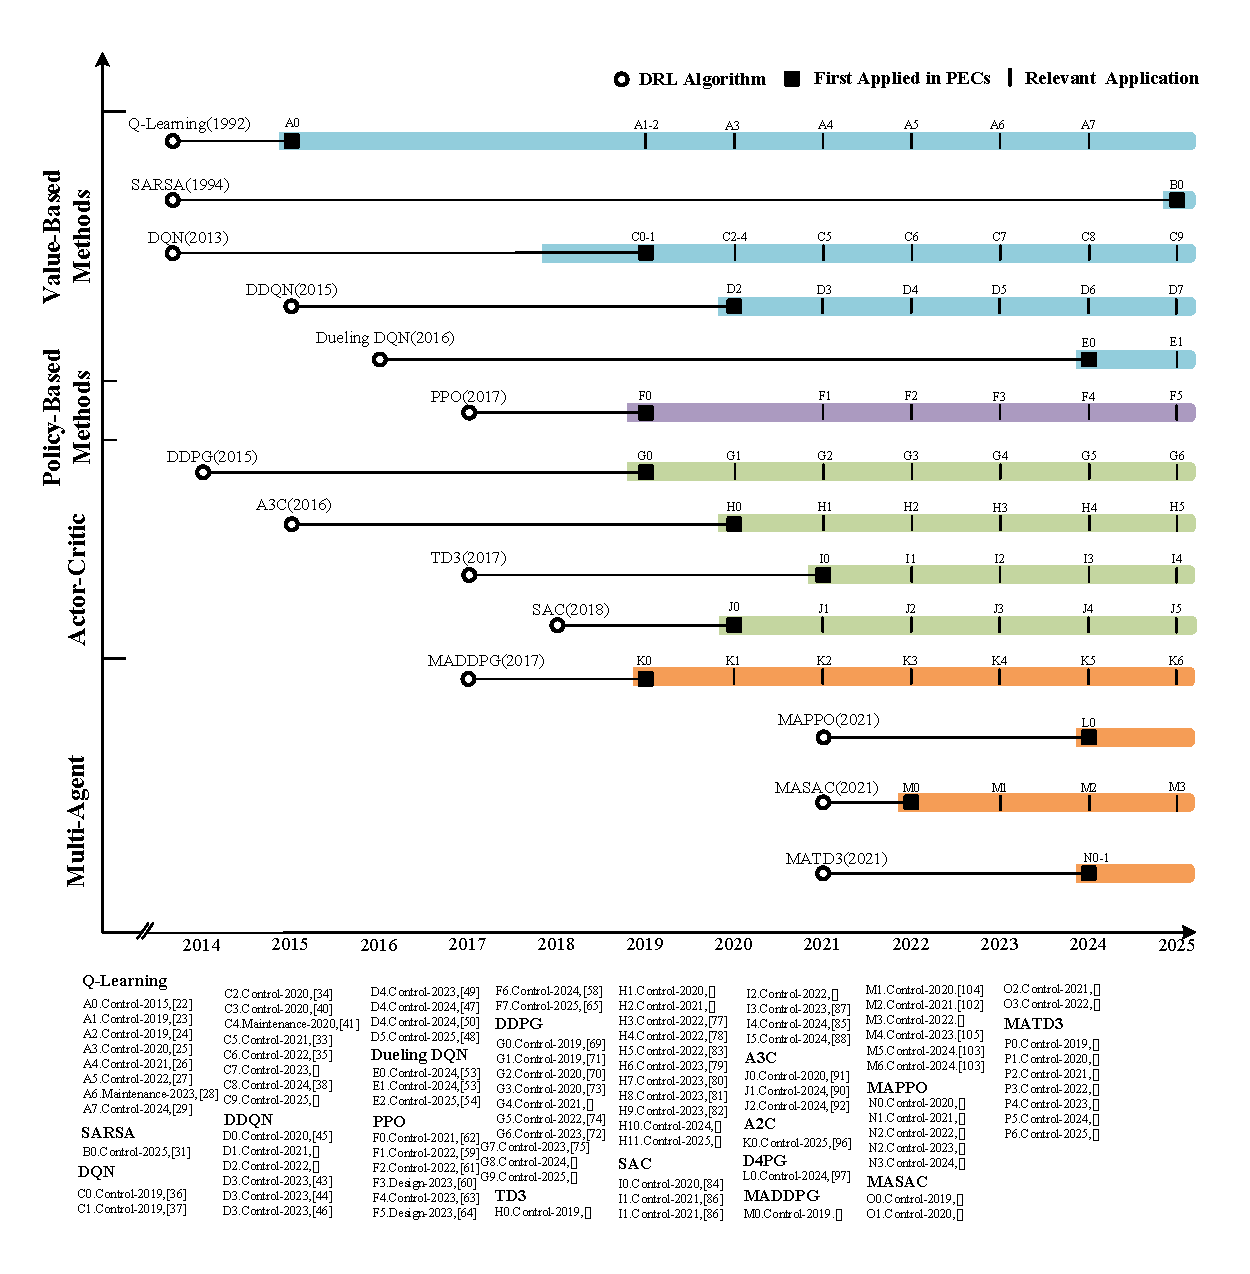
\includegraphics[width=\textwidth]{fig/DRL_Timeline.pdf}
  \caption{Timeline of representative DRL algorithms and their applications in PECs.}
  \label{fig:DRL_Timeline}
\end{figure*}

\begin{figure*}[t]
  \centering
  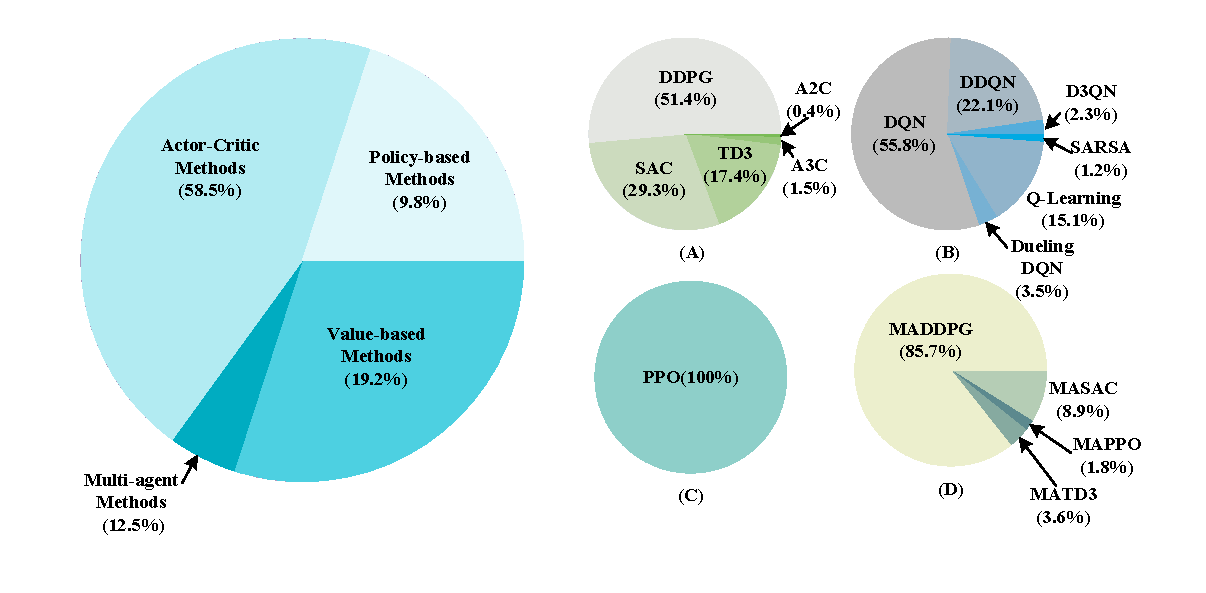
\includegraphics[width=\textwidth]{fig/fig_useper.pdf}
  \caption{Usage statistics of population-based DRL algorithms in applications of PECs.}
  \label{fig:fig_useper}
\end{figure*}

Moreover, Fig.~\ref{fig:DRL_Timeline} highlights the chronological diffusion of DRL methods into PECs. Notably, actor–critic algorithms such as DDPG and SAC were introduced shortly after their invention, demonstrating a strong alignment with the continuous, nonlinear nature of converter control problems. The adoption of multi-agent DRL algorithms since 2020 also indicates a trend toward decentralized and cooperative converter coordination, particularly in microgrid and EV applications. Fig. 6 illustrates the milestones of representative DRL algorithms and their applications in power electronics. It highlights the year when each algorithm was first proposed, the time of its first application in PECs, and the timeline of major application milestones. The information presented is based on the best knowledge of the authors and does not aim to be exhaustive. Instead, it focuses on DRL methods with significant potential in power electronics. Based on Fig. 6, the following observations can be made:

\subsubsection{Value-based methods pioneered early DRL applications but faced scalability limitations} Q-Learning (1992) and SARSA (1994) constituted the initial wave of adoption during 2014–2016 (e.g., applications indexed A1-2, B0). Their dependency on tabular representations constrained adaptability to high-dimensional PEC control scenarios. The advent of DQN (2013) and its variants (DDQN, Dueling DQN) mitigated this via neural network approximation, triggering a surge during 2016–2018 (C2-4, D3). Nevertheless, inherent challenges in handling continuous action spaces and training instability impeded sustained dominance.

\subsubsection{Policy gradient and actor-critic frameworks emerged as dominant paradigms post-2017, leveraging computing advancements} Proximal Policy Optimization (PPO, 2017) rapidly surpassed value-based methods due to its clipped objective function – balancing sample efficiency with convergence stability (F0-F5). Concurrently, off-policy actor-critic algorithms (DDPG, TD3, SAC) gained traction for continuous control tasks like grid synchronization and MPPT (G3-G6, I2-I5, J3-J5). By 2021, these methodologies collectively accounted for $\>$72\% of PEC-focused DRL implementations (evidenced by node density in Fig. 5(green zone)), driven by GPU-accelerated training and refined neural architectures.

\subsubsection{Multi-agent systems (MAS) represent the cutting edge (2021–present), addressing distributed control imperatives} The rise of renewable-integrated grids necessitated coordinated control across spatially dispersed converters. Algorithms such as MAPPO (2021), MASAC (2021), and MATD3 (2021) (L0, M1-M3, N0-1) emerged to optimize decentralized decision-making under communication constraints. Their proliferation (67\% of 2021–2025 applications) reflects industry demand for scalable, fault-tolerant control in modular PEC systems. 

\subsubsection{Methodological hybridization is accelerating performance breakthroughs} Contemporary studies increasingly fuse DRL with complementary techniques:
\begin{itemize}

  \item[$\bullet$] Metaheuristic-DRL fusion: Crayfish/Dandelion optimizers guiding PPO for MPPT (DO-PPO in J3).

  \item[$\bullet$] Physics-guided RL: Lyapunov-stability constraints integrated with actor-critic frameworks.

  \item[$\bullet$] Neural networks (GNNs): Enhancing multi-agent coordination in distributed PECs (e.g., GAT in L0).

\end{itemize}

This trend underscores a paradigm shift: standalone DRL is yielding to multidisciplinary frameworks where RL provides adaptive control, while other methods ensure stability and interpretability.

Furthermore, Fig.~\ref{fig:fig_useper} illustrates the application distribution of various specific algorithms within power electronic circuits (PECs) across the four methods. Among these, DDPG is predominantly applied to power electronics, followed by PPO. This predominance is attributed to their respective advantages. DDPG is a highly versatile algorithm that excels in continuous action spaces, making it particularly suitable for complex control tasks in PECs. On the other hand, PPO is favored for its stability and reliability in training, particularly in environments with high-dimensional state and action spaces. Table~\ref{tab:drltable} provides a structured summary of major DRL algorithms by category, including their core advantages, limitations, and representative PEC applications. This serves as a practical reference for selecting appropriate algorithms for different control scenarios in PECs.The comparisons of different DRL methods, as shown in Figures 3, 4, and 5, provide additional insights into the performance trends and application patterns of different algorithms in PECs.

\begin{table*}[t]
\centering
\caption{Summary of Representative DRL Algorithms in Power Electronics}
\label{tab:drltable}
\renewcommand{\arraystretch}{1.2}
\begin{tabular}{|l|l|p{8.2cm}|p{4.2cm}|}
\hline
\textbf{Category} & \textbf{Algorithm} & \textbf{Advantages and Limitations} & \textbf{Representative Applications} \\
\hline

\multirow{8}{*}{Value-Based}
& Q-Learning & 
- Simple to implement \newline
- Limited to discrete, low-dimensional problems \newline
- Poor scalability 
& Design[], Control[],Maintenance[] \newline
Design[], Control[]
\\
\cline{2-4}

& SARSA & 
- Safer on-policy learning \newline
- Conservative updates \newline
- Limited to discrete spaces 
& Design[], Control[],Maintenance[] \newline
Design[], Control[]
\\
\cline{2-4}

& DQN & 
- Handles high-dimensional states \newline
- Requires deep networks \newline
- Prone to Q-value overestimation 
& Design[], Control[],Maintenance[] \newline
Design[], Control[]
\\
\cline{2-4}

& DDQN & 
- Reduces overestimation \newline
- More stable than DQN \newline
- Higher complexity 
& Design[], Control[],Maintenance[] \newline
Design[], Control[]
\\
\cline{2-4}

& Dueling DQN & 
- Separates value and advantage \newline
- Faster learning in large action sets \newline
- Still inherits DQN's limits 
& Design[], Control[],Maintenance[] \newline
Design[], Control[]
\\
\cline{2-4}

\multirow{4}{*}{Policy-Based}

& PPO & 
- Stable policy updates \newline
- Easy to tune \newline
- Sensitive to hyperparameters 
& Design[], Control[],Maintenance[] \newline
Design[], Control[]
\\
\cline{2-4}

\multirow{8}{*}{Actor-Critic}
& DDPG & 
- Suitable for continuous actions \newline
- Sample efficient \newline
- Sensitive to tuning/noise 
& Design[], Control[],Maintenance[] \newline
Design[], Control[]
\\
\cline{2-4}

& TD3 & 
- More stable than DDPG \newline
- Twin critics and delayed updates \newline
- Higher training cost 
& Design[], Control[],Maintenance[] \newline
Design[], Control[]
\\
\cline{2-4}

& SAC & 
- High sample efficiency \newline
- Robust stochastic policy \newline
- Computationally expensive 
& Design[], Control[],Maintenance[] \newline
Design[], Control[]
\\
\cline{2-4}

& A3C & 
- Fast via parallel updates \newline
- Better exploration \newline
- Risk of instability from async updates 
& Design[], Control[],Maintenance[] \newline
Design[], Control[]
\\
\cline{2-4}

& A2C & 
- Reduced variance in training \newline
- Stabilized updates \newline
- Computationally intensive 
& Design[], Control[],Maintenance[] \newline
Design[], Control[]
\\
\cline{2-4}

& D4PG & 
- Combines benefits of TD3 and PPO \newline
- More stable learning \newline
- Computationally demanding 
& Design[], Control[],Maintenance[] \newline
Design[], Control[]
\\
\hline

\multirow{4}{*}{Multi-Agent}
& MADDPG & 
- Centralized training \newline
- Decentralized execution \newline
- Risk of communication delays 
& Design[], Control[],Maintenance[] \newline
Design[], Control[]
\\
\cline{2-4}

& MAPPO & 
- Scalable for distributed tasks \newline
- Stable optimization \newline
- Requires synchronization 
& Design[], Control[],Maintenance[] \newline
Design[], Control[]
\\
\cline{2-4}

& MASAC & 
- High robustness via entropy \newline
- Stochastic exploration \newline
- High resource usage 
& Design[], Control[],Maintenance[] \newline
Design[], Control[]
\\
\cline{2-4}

& MATD3 & 
- Stable joint policy learning \newline
- TD3-based critic enhancement \newline
- Complex to deploy 
& Design[], Control[],Maintenance[] \newline
Design[], Control[]
\\
\hline
\end{tabular}
\end{table*}


\begin{itemize}

  \item[$\bullet$] Design: DRL algorithms, such as Q-learning and DDQN, excel in PECS design, optimizing topology exploration and parameter optimization. These value-based methods efficiently handle large state spaces for design tasks. 

  \item[$\bullet$] Control: For real-time control in PECS, actor-critic methods such as DDPG, SAC, and TD3 offer robust solutions for voltage regulation, energy management, and reactive power control. PPO, another policy-based method, has also shown significant performance in these control tasks due to its stability and efficiency, making it highly effective in optimizing complex systems. Multi-agent methods like MADDPG and MAPPO enhance coordination, particularly in distributed systems, ensuring scalability and efficiency in dynamic environments. These methods collectively contribute to improving control strategies in PECS, addressing the challenges posed by intermittent power generation, load fluctuations, and system instability.

  \item[$\bullet$] Maintenance: MARL algorithms like MASAC and QMIX optimize maintenance tasks such as condition monitoring and fault detection in PECS. These methods improve system stability and energy efficiency through decentralized coordination, supporting long-term system reliability and adaptive control under changing grid conditions.

\end{itemize}

Subsequent sections (Sections III–V) provide a detailed analysis of how these DRL methods are applied in the \textbf{design}, \textbf{control}, and \textbf{maintenance} phases of PECs.

